\documentclass[a4paper,11pt,fleqn]{article}

\usepackage{layout}

\title{Power electronic systems - Exercise 5.5}
\author{Daniel Winz}
\date{\today}

\newcommand{\magmin}{0.000001}
\newcommand{\magmax}{10000}
\newcommand{\freqmin}{1000}
\newcommand{\freqmax}{1000000}
\newcommand{\angmin}{-360}
\newcommand{\angmax}{0}

\pgfplotsset{
    width=\linewidth,
    grid=minor,
    grid style={dashed,gray!30},
    every axis plot/.append style={ thick},
    legend cell align={left},
}

\begin{document}

\section{Exercise}
Given is the following boost converter: 

\begin{wrapfigure}{r}{0.7\textwidth}
    \centering
    \begin{circuitikz}[european voltages, european resistors, american inductors]
        \draw (0,0)
        to[V, v<=$V_i$]         +( 0, 2)
        to[short, i>^=$I_i$]    +( 1, 0)
        to[L=L, -*]             +( 2, 0)
        to[D, l=D, -*]          +( 2, 0)
        to[short, i>^=$I_o$]    +( 2, 0)
        to[R=R]                 +( 0,-2)
        to[short, -*]           +(-2, 0)
        to[short, -*]           +(-2, 0)
        to[short]               +(-3, 0)
        (5, 2) to[C=C]          (5,0)
        (3,1) node[nigfete=Q] (fet) {}
        (fet) node[right] {Q}
        (fet.S) to[short] (3,0)
        (fet.D) to[short] (3,2)
        (7.5,2) to[open, v^>=$V_0$] (7.5,0)
        ;
    \end{circuitikz}
\end{wrapfigure}

\[ V_o = \SI{200}{\volt} \]
\[ L = \SI{200}{\micro\henry} \]
\[ C = \SI{5}{\micro\farad} \]
\[ R = \SI{50}{\ohm} \]
\[ f_s = \SI{100}{\kilo\hertz} \]

\section{Solution}
%\begin{table}[h!]
\begin{wraptable}{r}{0.25\textwidth}
    \centering
    \begin{zebratabular}{lll}
        \rowcolor{gray}
        $V_i$ [\si{\volt}]  & $V_o$ [\si{\volt}]    & $D$ [\,]\\
         50 & 200   & 0.75  \\
        100 & 200   & 0.5   \\
        150 & 200   & 0.25  \\
    \end{zebratabular}
    \caption{Duty cycle for several input voltages}
    \label{tab:duty}
\end{wraptable}
The duty ratio for different input voltages is calculated using the volt 
second balance. 
\[ V_{L_1} \cdot D + V_{L_2} \cdot (1 - D) = 0 \]
\[ V_{L_1} = V_i \qquad V_{L_2} = V_i - V_o \]
\[ \to V_i \cdot D + (V_i - V_o) \cdot (1 - D) = 0 \]
\[ V_i \cdot D + V_i \cdot (1 - D) - V_o \cdot (1 - D) = 0 \]
\[ V_i \cdot \underbrace{(D + 1 - D)}_{1} = V_o \cdot (1 - D) \]
%\[ V_o = \dfrac{V_i}{1 - D} \]
%\[ M(D) = \dfrac{V_o}{V_i} = \dfrac{1}{1 - D} \]
\[ \underline{D = 1 - \dfrac{V_i}{V_o}} \]

%\begin{figure}[h!]
\begin{wrapfigure}{r}{0.5\textwidth}
    \centering
    %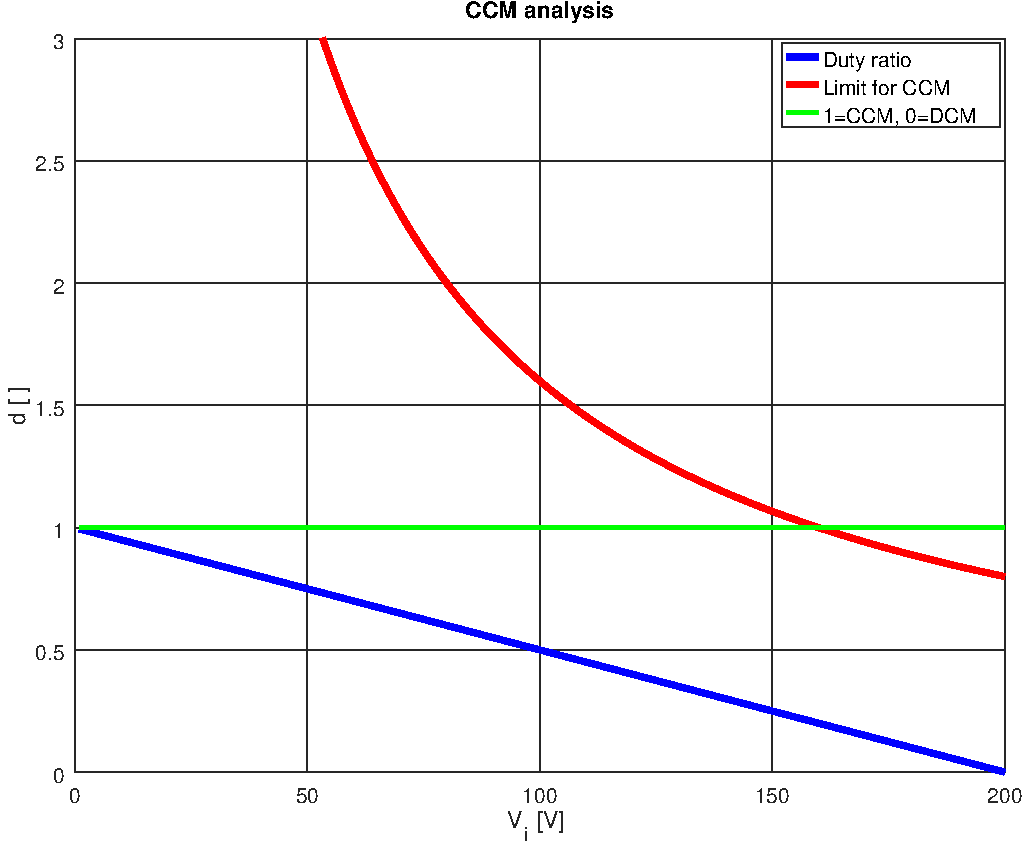
\includegraphics[width=0.8\textwidth]{fig/ccm.pdf}
    \begin{tikzpicture}
        \begin{axis}[
            width=0.5\textwidth,
            title=\textbf{CCM Analysis},
            xlabel={$V_i$ [\si{\volt}]},
            ylabel={$d$},
            grid=major,
            ymin=0,
            ymax=2,
            restrict y to domain=0:10,
            xmin=0,
            xmax=200,
            ]
            \addplot+[mark=none] table[x=vi, y=d, col sep=comma, blue]{data/ccm.csv};
            \addlegendentry{Duty ratio};
            \addplot+[mark=none] table[x=vi, y=dmax, col sep=comma, red]{data/ccm.csv};
            \addlegendentry{Limit for CCM};
            %\addplot+[mark=none] table[x=vi, y=ccm, col sep=comma, green]{data/ccm.csv};
            %\addlegendentry{1=CCM, 0=DCM};
            %\draw[] (axis cs: 20,0.5) -- (axis cs: 80,0.5);
        \end{axis}
    \end{tikzpicture}
    \caption{CCM analysis over complete input voltage range}
    \label{fig_ccm}
\end{wrapfigure}
%\end{figure}

For each input voltage it is checked, if the converter is still in continuous 
conduction mode (CCM). 
\[ \Delta I_L < 2 \cdot I_o \]
\[ \dfrac{V_i \cdot D}{L \cdot f_s} < 2 \cdot \dfrac{V_o}{R} \]
\[ D < 2 \cdot \dfrac{V_o \cdot L \cdot f_s}{R \cdot V_i} \]

To determine the transfer function of the converter state-space-averaging is used. The State variables are the inductor current $i_L$ and the output capacitor voltage $v_c$. 
\[ X = \begin{bmatrix}i_L\\v_c\end{bmatrix} \]
The output voltage is equal to the capacitor voltage. 
\[ F = \begin{bmatrix}0 & 1\end{bmatrix} \]
\[ v_o = F \cdot X \]

\begin{multicols}{2}
    \subsubsection*{Interval 1:}
        \begin{circuitikz}[scale=0.9, european voltages, european resistors, american inductors]
            \draw (0,0)
            to[V, v<=$V_i$]         +( 0, 2)
            to[short, i>^=$I_i$]    +( 1, 0)
            to[L=L]                 +( 2, 0)
            to[open]                +( 2, 0)
            to[short, i>^=$I_o$]    +( 2, 0)
            to[R=R]                 +( 0,-2)
            to[short, -*]           +(-2, 0)
            to[short, -*]           +(-2, 0)
            to[short]               +(-3, 0)
            (5, 2) to[C=C]          (5,0)
            (3,0) to[short] (3,2)
            (7.5,2) to[open, v^>=$V_0$] (7.5,0)
            ;
        \end{circuitikz}
    \[ \dfrac{di_L}{dt} = \dfrac{v_L}{L} = \dfrac{v_i}{L} \]
    \[ \dfrac{dv_C}{dt} = \dfrac{i_C}{C} = \dfrac{-i_o}{C} = \dfrac{-v_c}{R \cdot C} \]
    \[ \underbrace{
        \begin{bmatrix}
            \dfrac{di_L}{dt} \\
            \dfrac{dv_C}{dt}
        \end{bmatrix}}_{\dot{x}} 
    = 
        \underbrace{
        \begin{bmatrix}
            0 & 0 \\
            0 & \dfrac{-1}{R \cdot C}
        \end{bmatrix}}_{A_1} 
    \cdot
        \underbrace{
        \begin{bmatrix}
            i_L \\
            v_C
        \end{bmatrix}}_{x} 
    +
        \underbrace{
        \begin{bmatrix}
            \dfrac{v_i}{L} \\
            0
        \end{bmatrix}}_{B_1} 
    \]
    \[ \dot{x} = A_1 \cdot x + B_1 \]
\columnbreak
    \subsubsection*{Interval 2:}
        \begin{circuitikz}[scale=0.9, european voltages, european resistors, american inductors]
            \draw (0,0)
            to[V, v<=$V_i$]         +( 0, 2)
            to[short, i>^=$I_i$]    +( 1, 0)
            to[L=L]                 +( 2, 0)
            to[short, -*]           +( 2, 0)
            to[short, i>^=$I_o$]    +( 2, 0)
            to[R=R]                 +( 0,-2)
            to[short, -*]           +(-2, 0)
            to[short]               +(-2, 0)
            to[short]               +(-3, 0)
            (5, 2) to[C=C]          (5,0)
            (7.5,2) to[open, v^>=$V_0$] (7.5,0)
            ;
        \end{circuitikz}
    \[ \dfrac{di_L}{dt} = \dfrac{v_L}{L} = \dfrac{v_i - v_c}{L} \]
    \[ \dfrac{dv_C}{dt} = \dfrac{i_C}{C} = \dfrac{i_L - i_o}{C} = \dfrac{i_L}{C} - \dfrac{v_c}{R \cdot C} \]
    \[ \underbrace{
        \begin{bmatrix}
            \dfrac{di_L}{dt} \\
            \dfrac{dv_C}{dt}
        \end{bmatrix}}_{\dot{x}} 
    = 
        \underbrace{
        \begin{bmatrix}
            0 & \dfrac{-1}{L} \\
            \dfrac{1}{C} & \dfrac{-1}{R \cdot C}
        \end{bmatrix}}_{A_2} 
    \cdot
        \underbrace{
        \begin{bmatrix}
            i_L \\
            v_C
        \end{bmatrix}}_{x} 
    +
        \underbrace{
        \begin{bmatrix}
            \dfrac{v_i}{L} \\
            0
        \end{bmatrix}}_{B_2} 
    \]
    \[ \dot{x} = A_2 \cdot x + B_2 \]
\end{multicols}
\vspace{-1cm}
\[ D' = 1 - D \qquad D + D' = 1 \]
\[ A = A_1 \cdot D + A_2 \cdot D'
     = \begin{bmatrix}
            0 & 0 \\
            0 & \dfrac{-1}{R \cdot C}
        \end{bmatrix}
     \cdot D
     + \begin{bmatrix}
            0 & \dfrac{-1}{L} \\
            \dfrac{1}{C} & \dfrac{-1}{R \cdot C}
        \end{bmatrix}
     \cdot D'
     = \begin{bmatrix}
            0 & \dfrac{-D'}{L} \\
            \dfrac{D'}{C} & \dfrac{-1}{R \cdot C}
        \end{bmatrix}
     = \begin{bmatrix}
            0 & \dfrac{D-1}{L} \\
            \dfrac{1-D}{C} & \dfrac{-1}{R \cdot C}
        \end{bmatrix}
\]
\[ B = B_1 \cdot D + B_2 \cdot D'
     = \begin{bmatrix}
            \dfrac{v_i}{L} \\
            0
        \end{bmatrix}
     \cdot D 
     + \begin{bmatrix}
            \dfrac{v_i}{L} \\
            0
        \end{bmatrix}
     \cdot D'
     = \begin{bmatrix}
            \dfrac{v_i}{L} \\
            0
        \end{bmatrix}
\]
\[ X = \begin{bmatrix}i_L\\v_c\end{bmatrix} = -A^{-1} \cdot B 
     = -\begin{bmatrix}
            \dfrac{-L}{(D - 1)^2 \cdot R} & \dfrac{-C}{D - 1} \\
            \dfrac{L}{D-1} & 0
        \end{bmatrix} \cdot B
     = \begin{bmatrix}
            \dfrac{v_i}{(D - 1)^2 \cdot R} \\
            \dfrac{-v_i}{D-1}
        \end{bmatrix}
\]
\[ E = (A_1 - A_2) \cdot X + B_1 - B_2
     = \begin{bmatrix}
            \dfrac{v_c}{L} \\
            \dfrac{-i_l}{C}
        \end{bmatrix}
\]
\[ H(s) = \dfrac{\hat{V}_o(s)}{\hat{D}(s)} = F \cdot (s \cdot I - A)^{-1} \cdot E
    = \dfrac{\dfrac{v_C}{1 - D} - \dfrac{L \cdot i_L}{(1 - D)^2} \cdot s}
        {1 + \dfrac{L}{R \cdot (1 - D)^2} \cdot s + \dfrac{C \cdot L}{(1 - D)^2} \cdot s^2}
\]
\[ v_C = v_o \qquad i_L = \dfrac{v_o}{(1 - D) \cdot R} \]
\[ H(s) = \dfrac{\dfrac{v_o}{1 - D} - \dfrac{L \cdot v_o}{(1 - D)^3 \cdot R} \cdot s}
        {1 + \dfrac{L}{R \cdot (1 - D)^2} \cdot s + \dfrac{C \cdot L}{(1 - D)^2} \cdot s^2}
    = \dfrac{v_o}{1 - D} \cdot \dfrac{1 - \dfrac{L}{(1 - D)^2 \cdot R} \cdot s}
        {1 + \dfrac{L}{R \cdot (1 - D)^2} \cdot s + \dfrac{C \cdot L}{(1 - D)^2} \cdot s^2}
\]

\clearpage

\begin{figure}[h!]
    \begin{subfigure}[b]{0.9\textwidth}
        \centering
        \begin{tikzpicture}
            \begin{axis}[
                xmode=log,
                ymode=log,
                height=0.45\textwidth,
                title=\textbf{Magnitude},
                xlabel={$\omega [\si{\per\second}]$},
                ylabel={$|H| \, [\si{\decibel}]$},
                ymin=\magmin,
                ymax=\magmax,
                xmin=\freqmin,
                xmax=\freqmax,
                ]
                \addplot+[mark=none] table[x=angfreq, y=magnitude, col sep=comma]{data/bode_h1.csv};
                \addlegendentry{$V_i = \SI{50}{\volt}$};
                \addplot+[mark=none] table[x=angfreq, y=magnitude, col sep=comma]{data/bode_h2.csv};
                \addlegendentry{$V_i = \SI{100}{\volt}$};
                \addplot+[mark=none] table[x=angfreq, y=magnitude, col sep=comma]{data/bode_h3.csv};
                \addlegendentry{$V_i = \SI{150}{\volt}$};
                %\draw[] (axis cs: 20,0.5) -- (axis cs: 80,0.5);
            \end{axis}
        \end{tikzpicture}
    \end{subfigure}
    \begin{subfigure}[b]{0.9\textwidth}
        \centering
        \begin{tikzpicture}
            \begin{axis}[
                xmode=log,
                ymode=linear,
                height=0.45\textwidth,
                title=\textbf{Phase},
                xlabel={$\omega [\si{\per\second}]$},
                ylabel={$\varphi(H) \, [\si{\degree}]$},
                ymin=\angmin,
                ymax=\angmax,
                xmin=\freqmin,
                xmax=\freqmax,
                ]
                \addplot+[mark=none] table[x=angfreq, y=phase, col sep=comma]{data/bode_h1.csv};
                \addlegendentry{$V_i = \SI{50}{\volt}$};
                \addplot+[mark=none] table[x=angfreq, y=phase, col sep=comma]{data/bode_h2.csv};
                \addlegendentry{$V_i = \SI{100}{\volt}$};
                \addplot+[mark=none] table[x=angfreq, y=phase, col sep=comma]{data/bode_h3.csv};
                \addlegendentry{$V_i = \SI{150}{\volt}$};
                \draw[red, dashed, thick] (axis cs: 1000,-120) -- (axis cs: 1000000,-120);
            \end{axis}
        \end{tikzpicture}
    \end{subfigure}
    \caption{Magnitude and phase of converter}
    \label{fig:bode_h}
\end{figure}

\clearpage

As controller a PI controller with the following parameters is chosen. The 
parameter have been evaluated by iterating $K_P$ and $\omega_i$ so that the 
step response shows no significant overshoot with all three evaluated input 
voltages. 
\[ G(s) = K_P \cdot \left(1 + \dfrac{\omega_i}{s}\right) \qquad | K_p = 9\cdot 10^{-9}, \quad \omega_i = 200 \cdot 10^{3} \si{\per\second} \]
\begin{figure}[h!]
    \begin{subfigure}[b]{0.9\textwidth}
        \centering
        \begin{tikzpicture}
            \begin{axis}[
                xmode=log,
                ymode=log,
                height=0.45\textwidth,
                title=\textbf{Magnitude},
                xlabel={$\omega [\si{\per\second}]$},
                ylabel={$|G| \, [\si{\decibel}]$},
                ymin=\magmin,
                ymax=\magmax,
                xmin=\freqmin,
                xmax=\freqmax,
                ]
                \addplot+[mark=none] table[x=angfreq, y=magnitude, col sep=comma]{data/bode_g.csv};
                %\addlegendentry{$V_i = \SI{50}{\volt}$};
                %\addplot+[mark=none] table[x=angfreq, y=magnitude, col sep=comma]{data/bode_h2.csv};
                %\addlegendentry{$V_i = \SI{100}{\volt}$};
                %\addplot+[mark=none] table[x=angfreq, y=magnitude, col sep=comma]{data/bode_h3.csv};
                %\addlegendentry{$V_i = \SI{150}{\volt}$};
                %\draw[] (axis cs: 20,0.5) -- (axis cs: 80,0.5);
            \end{axis}
        \end{tikzpicture}
    \end{subfigure}
    \begin{subfigure}[b]{0.9\textwidth}
        \centering
        \begin{tikzpicture}
            \begin{axis}[
                xmode=log,
                ymode=linear,
                height=0.45\textwidth,
                title=\textbf{Phase},
                xlabel={$\omega [\si{\per\second}]$},
                ylabel={$\varphi(G) \, [\si{\degree}]$},
                ymin=\angmin,
                ymax=\angmax,
                xmin=\freqmin,
                xmax=\freqmax,
                ]
                \addplot+[mark=none] table[x=angfreq, y=phase, col sep=comma]{data/bode_g.csv};
                %\addlegendentry{$V_i = \SI{50}{\volt}$};
                %\addplot+[mark=none] table[x=angfreq, y=phase, col sep=comma]{data/bode_h2.csv};
                %\addlegendentry{$V_i = \SI{100}{\volt}$};
                %\addplot+[mark=none] table[x=angfreq, y=phase, col sep=comma]{data/bode_h3.csv};
                %\addlegendentry{$V_i = \SI{150}{\volt}$};
                %\draw[red, dashed, thick] (axis cs: 1000,-120) -- (axis cs: 1000000,-120);
            \end{axis}
        \end{tikzpicture}
    \end{subfigure}
    \caption{Magnitude and phase of controller}
    \label{fig:bode_g}
\end{figure}

\clearpage

\begin{figure}[h!]
    \begin{subfigure}[b]{0.9\textwidth}
        \centering
        \begin{tikzpicture}
            \begin{axis}[
                xmode=log,
                ymode=log,
                height=0.45\textwidth,
                title=\textbf{Magnitude},
                xlabel={$\omega [\si{\per\second}]$},
                ylabel={$|G \cdot H| \, [\si{\decibel}]$},
                ymin=\magmin,
                ymax=\magmax,
                xmin=\freqmin,
                xmax=\freqmax,
                ]
                \addplot+[mark=none] table[x=angfreq, y=magnitude, col sep=comma]{data/bode_gh1.csv};
                \addlegendentry{$V_i = \SI{50}{\volt}$};
                \addplot+[mark=none] table[x=angfreq, y=magnitude, col sep=comma]{data/bode_gh2.csv};
                \addlegendentry{$V_i = \SI{100}{\volt}$};
                \addplot+[mark=none] table[x=angfreq, y=magnitude, col sep=comma]{data/bode_gh3.csv};
                \addlegendentry{$V_i = \SI{150}{\volt}$};
                %\draw[] (axis cs: 20,0.5) -- (axis cs: 80,0.5);
            \end{axis}
        \end{tikzpicture}
    \end{subfigure}
    \begin{subfigure}[b]{0.9\textwidth}
        \centering
        \begin{tikzpicture}
            \begin{axis}[
                xmode=log,
                ymode=linear,
                height=0.45\textwidth,
                title=\textbf{Phase},
                xlabel={$\omega [\si{\per\second}]$},
                ylabel={$\varphi(G \cdot H) \, [\si{\degree}]$},
                ymin=\angmin,
                ymax=\angmax,
                xmin=\freqmin,
                xmax=\freqmax,
                ]
                \addplot+[mark=none] table[x=angfreq, y=phase, col sep=comma]{data/bode_gh1.csv};
                \addlegendentry{$V_i = \SI{50}{\volt}$};
                \addplot+[mark=none] table[x=angfreq, y=phase, col sep=comma]{data/bode_gh2.csv};
                \addlegendentry{$V_i = \SI{100}{\volt}$};
                \addplot+[mark=none] table[x=angfreq, y=phase, col sep=comma]{data/bode_gh3.csv};
                \addlegendentry{$V_i = \SI{150}{\volt}$};
                \draw[red, dashed, thick] (axis cs: 1000,-120) -- (axis cs: 1000000,-120);
            \end{axis}
        \end{tikzpicture}
    \end{subfigure}
    \caption{Magnitude and phase of open loop system}
    \label{fig:bode_gh}
\end{figure}

\clearpage

\begin{figure}[h!]
    \centering
    \begin{tikzpicture}
        \begin{axis}[
            title=\textbf{Step response},
            xlabel={$t [\si{\milli\second}]$},
            ylabel={$d$},
            grid=major,
            ymin=-0.02,
            ymax=1.02,
            xmin=0,
            xmax=10,
            ]
            \addplot+[mark=none] table[x=t, y=y, col sep=comma]{data/step_gh1.csv};
            \addlegendentry{$V_i = \SI{50}{\volt}$};
            \addplot+[mark=none] table[x=t, y=y, col sep=comma]{data/step_gh2.csv};
            \addlegendentry{$V_i = \SI{100}{\volt}$};
            \addplot+[mark=none] table[x=t, y=y, col sep=comma]{data/step_gh3.csv};
            \addlegendentry{$V_i = \SI{150}{\volt}$};
            %\draw[red, dashed, thick] (axis cs: 1000,-120) -- (axis cs: 1000000,-120);
        \end{axis}
    \end{tikzpicture}
    \caption{Step response of closed loop system}
    \label{fig:step_gh}
\end{figure}

\clearpage

\appendix
\section{Octave Code}
All code for above calculations and plots is listed below. All scripts for 
this attestation together with the sources for this documentation are also 
available on \url{https://github.com/daniw/powelsys}. In order to compile the 
documentation the script \verb!pes_att.m! has to be run with Octave or Matlab 
to generate the data needed for the plots. 
\lstsettingm
\lstinputlisting{pes_att.m}

\end{document}
